\section{Optimisation: The Role of Depth}\label{sec:optimisation}
\begin{comment}
Consider a DNN with ReLU activation at time $t$. Now, by collecting the gating values for the $n$ examples in the dataset in $\G_t$, we can define the NPF matrix $\Phi_t=(\phi_{x_s,t},s\in[n] )\in \R^{d_{net}\times n}$. In the case of say \emph{squared-loss}, GD considers the following problem:
\begin{align}
\min_{\Theta\inrdnet}\norm{\Phi^\top_tv_{\Theta_t+\Theta}-y}_2^2,
\end{align}
\end{comment}
The error trajectory of the GD is then given by $e_{t+1}=e_t-\alpha_t K_te_t$, where $e_t=(\hat{y}_t(x_s)-y_s,s\in[s])\in\R^n$, and $K_t=\Psi^\top_t\Psi_t$, with $\Psi_t$ being the $d_{net}\times n$ NTF matrix. Now, $\Psi_t$ is given by $\Psi_t=\left(\nabla_{\Theta|_{\Theta=\Theta_t}v_t}\right)^\top\Phi_t$, where $\nabla_{\Theta}v_t=$ is a $P\times d_{net}$ matrix of $\partial_{\theta} v_t(p),\forall p\in [P], \theta\in \Theta$. Putting together, we have:
\begin{align*}
K_t=\Psi^\top_t\Psi_t=\Phi^\top_t\left(\nabla_{\Theta|_{\Theta=\Theta_t}v_t}\right)\left(\nabla_{\Theta|_{\Theta=\Theta_t}v_t}\right)^\top\Phi_t
\end{align*}
At $t=0$, using \Cref{assmp:init,assmp:decouple}, we can obtain the following simplified expression
\begin{align}\label{eq:opti-refer}
\E{K_0}=\Phi^\top_t\E{\left(\nabla_{\Theta|_{\Theta=\Theta_t}v_t}\right)\left(\nabla_{\Theta|_{\Theta=\Theta_t}v_t}\right)^\top}\Phi_t=d\sigma^{2(d-1)}(x^\top x)\odot \lambda_0
\end{align}
\textbf{Role of Randomisation:} Note that, in \Cref{assmp:decouple} helps us in pulling out the $\Phi^\top_t$ and $\Phi_t$ terms outside, and \Cref{assmp:init} disentangles the path as per \Cref{lm:disentangle}, due to which the inner expectation of $\nabla_{\Theta}v\nabla^\top_{\Theta}v$ reduces to a $P\times P$ identity matrix times a constant $d\sigma^{2(d-1)}$.\\
\textbf{Active Sub-Network and Gradient Flow:}  Each input example has its own associated set of active sub-network, and while training a particular example, the gradient flows through the weights of the corresponding active sub-network. Now, the active sub-networks corresponding to different examples have some overlap, and hence there is bound to be \emph{cross-talk} of the gradients flowing through them. This overlap is captured by $\lambda_t(s,s')$ which is the measure of overlap of the sub-networks that are active for both the inputs $x,x'\in\R^{d_{in}}$. As seen from \Cref{th:main}, $\lambda_0$ directly controls the spectral properties of the NTK matrix $K_0$.\\
\textbf{Why increasing depth till a point helps in training? } From \Cref{th:main}-(ii) it follows that for $w\ra\infty$, $K_0\ra\E{K_0}$. We now argue that when $\sigma=\sqrt{\frac{2}{w}}$, increasing depth causes whitening of $\lambda_0$, and hence $K_0$ .\hfill\\
$1.$ Let us first look at the diagonal terms of $\lambda_0$. It is reasonable to assume that, owing to the symmetric nature of the weights, roughly $\mu=\frac{1}{2}$ fraction of the gates are \emph{on} every layer. Thus $\lambda_0(s,s)\approx (w/2)^{d-1}$. Now, due our choice of $\sigma=\sqrt{\frac{2}{w}}$, the diagonal entries will be close to $1$.\hfill\\
$2.$ We now turn our attention towards the non-diagonal entries of $\lambda_0$. Define $\tau(s,s',l)\stackrel{def}=\sum_{i=1}^w G_{x_s,t}(l,i)G_{x_{s'},t}(l,i)$ be the overlap of the active gates in layer $l$ for input examples $s,s'\in[n]$, and  let $\eta\stackrel{def}=\max_s\left(\max_{s',l} \frac{\tau(s,s',l)}{\tau(s,s,l)}\right)$ be the maximum overlap between gates of a layer (maximum taken over over input pairs $s,s'\in[n]$ and layers $l\in [d]$).  Then it follows that $\max_{s,s'\in [n]} \frac{\bar{\lambda}_{cross}(s,s')}{\bar{\lambda}_{self}(s)}\leq \eta^{d-1}$. Thus, the non-diagonal entries decay an exponential rate in comparison to the diagonal entries.\hfill\\
\textbf{Why increasing the depth beyond hurts training?} Note that for $\sigma=O\left(\sqrt{\frac{1}{w}}\right)$, for a fixed depth $d$, as width $w$ increases, $K_0\ra\E{K_0}$. However, the variance expression in \Cref{th:main}-$(ii)$ involves $d^2$ and $d^3$ terms, and hence for a fixed width as depth increases, the entries of $K_0$ deviates from $\E{K_0}$, and as a result the spectrum of $K_0$ degrades, thereby hurting training performance.
\textbf{Closed form expression for $\lambda_0$ (fixed random gates):} 
Consider the dataset $(x_s,y_s)_{s=1}^n\in \R\times \R$, where $x_s=1,\forall s\in [n]$, and $y_s\sim unif([-1,1])$, $n=200$. The input Gram matrix $x^\top x$ is a $n\times n$ matrix with all entries equal to $1$ and its rank is equal to 1. Since all the inputs are identical, this is the worst possible case for optimisation. In this experiment, since we are interested only in the optimisation question, we take full control of the gating. For each input example, we sample gating values from $Ber(\mu)$ taking values in $\{0,1\}$, and collect it in $\G_0$. In this case, it is easy to check that $\mathbf{E}_{\mu}\left[\lambda_0(s,s)\right]=(\mu w)^{(d-1)},\forall s\in[n]$ and $\mathbf{E}_{\mu}\left[\lambda_0(s,s')\right]=(\mu^2 w)^{(d-1)},\forall s,s'\in[n]$.\hfill\\
\textbf{Theoretical Prediction:} It follows that,  for $\sigma=\sqrt{\frac{1}{\mu w}}$, all the diagonal entries of $\E{K_0}/d$ are $1$ and non-diagonal entries are $\mu^{d-1}$. Now, let $\rho_i\geq 0,i \in [n]$ be the eigenvalues of $\frac{\E{K_0}}{d}$, and let $\rho_{\max}$ and $\rho_{\min}$ be the largest and smallest eigenvalues.  One can easily show that $\rho_{\max}=1+(n-1)\mu^{d-1}$ and corresponds to the eigenvector with all entries as $1$, and $\rho_{\min}=(1-\mu^{d-1})$ repeats $(n-1)$ times, which corresponds to eigenvectors given by $[0, 0, \ldots, \underbrace{1, -1}_{\text{$i$ and $i+1$}}, 0,0,\ldots, 0]^\top \in \R^n$ for $i=1,\ldots,n-1$.\hfill\\
\begin{figure*}
\resizebox{\textwidth}{!}{
\begin{tabular}{ccc}
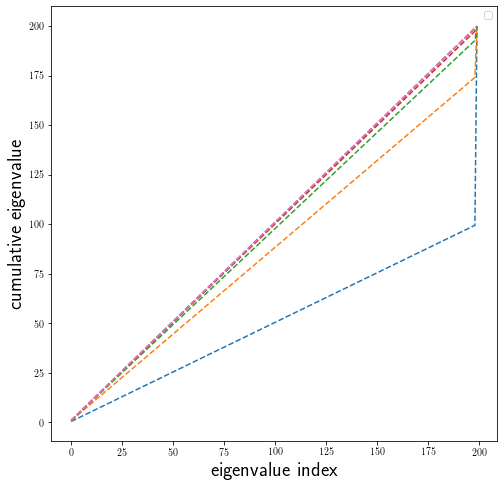
\includegraphics[scale=0.4]{figs/dgn-fra-ecdf-ideal.png}
&
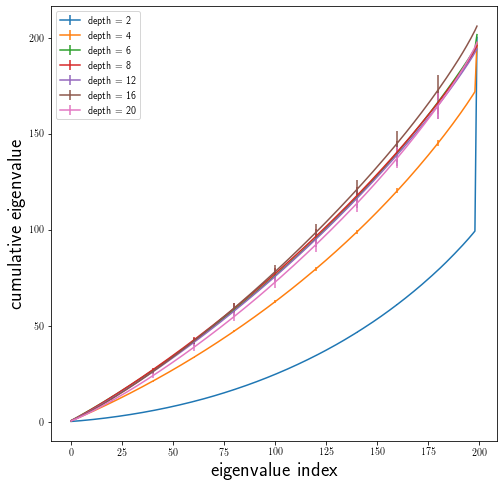
\includegraphics[scale=0.4]{figs/dgn-fra-ecdfbyd-w500.png}
&
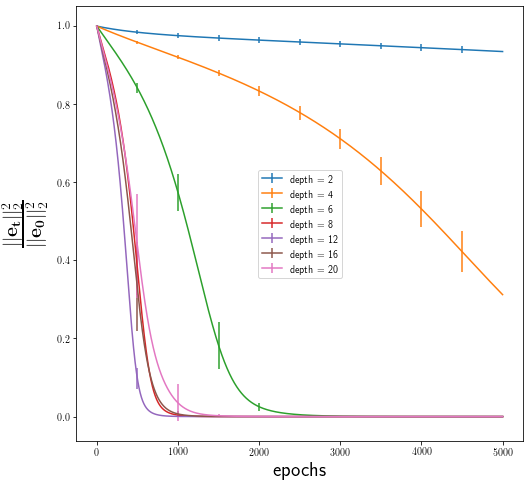
\includegraphics[scale=0.4]{figs/dgn-fra-conv-w500.png}
\end{tabular}
}
\caption{Shows the plots for DGN-FRG with $\mu=\frac{1}{2}$ and $\sigma=\sqrt{\frac{2}{w}}$. The first plot in the left shows the ideal cumulative eigenvalue (e.c.d.f) for various depths $d=2,4,6,8,12,16,20$. Note that the ideal plot converges to identity matrix as $d$ increases. The second plot from the left shows the cumulative eigenvalues (e.c.d.f) for $w=500$. }
\label{fig:dgn-frg-gram-ecdf}
\end{figure*}
\textbf{Numerical Evidence:} We look at the cumulative eigenvalue (e.c.d.f) obtained by first sorting the eigenvalues in ascending order then looking at their cumulative sum. The ideal behaviour (middle plot of \Cref{fig:dgn-frg-gram-ecdf}) as predicted from theory is that for indices $k\in[n-1]$, the e.c.d.f should increase at a linear rate, i.e., the cumulative sum of the first $k$ indices is equal to $k(1-\mu^{d-1})$, and the difference between the last two indices is $1+(n-1)\mu^{d-1}$. In \Cref{fig:dgn-frg-gram-ecdf}, we plot the e.c.d.f for various depths $d=2,4,6,8,12,16,20$ and $w=500$. \hfill\\
In order to compare how the rate of convergence varies with the depth, we set the step-size $\alpha=\frac{0.1}{\rho_{\max}}$, $w=100$. We use the vanilla SGD-optimiser. Note that the convergence rate is determined by a linear recursion $e_{t+1}=e_t-\alpha_t K_te_t$, and choosing $\alpha=\frac{0.1}{\rho_{\max}}$ can be seen to be equivalent to having a constant step-size of $\alpha=0.1$ but dividing the Gram matrix by its maximum eigenvalue instead. Thus, after this rescaling, the maximum eigenvalue is $1$ uniformly across all the instances, and the convergence should be limited by the smaller eigenvalues. We also look at the convergence rate of the ratio $\frac{\norm{e_t}^2_2}{\norm{e_0}^2_2}$, and we observe that the convergence rate gets better with depth as predicted by theory.
